\documentclass[]{article}

% Imported Packages
%------------------------------------------------------------------------------
\usepackage{amssymb}
\usepackage{amstext}
\usepackage{amsthm}
\usepackage{amsmath}
\usepackage{enumerate}
\usepackage{fancyhdr}
\usepackage[margin=1in]{geometry}
\usepackage{graphicx}
\usepackage{extarrows}
\usepackage{setspace}
\usepackage{float}
%------------------------------------------------------------------------------

% Header and Footer
%------------------------------------------------------------------------------
\pagestyle{plain}  
\renewcommand\headrulewidth{0.4pt}                                      
\renewcommand\footrulewidth{0.4pt}                                    
%------------------------------------------------------------------------------

% Title Details
%------------------------------------------------------------------------------
\title{Deliverable \#3: What’s That Dish Software}
\author{SE 3A04: Software Design II -- Large System Design}
\date{}                               
%------------------------------------------------------------------------------

% Document
%------------------------------------------------------------------------------
\begin{document}

\maketitle	
\noindent{\bf Tutorial Number:} T03\\
{\bf Group Number:} G03 \\
{\bf Group Members:} 
\begin{itemize}
	\item Imran Chowdhury
	\item Michael Roberts
	\item Sathurshan Arulmohan
	\item Tanisha Tasnin
	\item Zifan Si
\end{itemize}

\section{Introduction}
\label{sec:introduction}
% Begin Section

This section should provide an brief overview of the entire document.

\subsection{Purpose}
\label{sub:purpose}
% Begin SubSection

This document provides further detail on the architecure and design of \textit{What's that Dish}, including state diagrams for controller classes,
sequence diagrams and the detailed class diagram. It compliments Deliverables 1 and 2, which all readers are advised to familarize themselves with
to further their understanding of this document.

This document is intended for internal technical stakeholders, including, but not limited to, developers, domain experts,
and engineering managers. It may have some use to non-technical stakeholders, including non-engineering project managers,
senior executives, investors, restarants, and future end users.
% End SubSection

\subsection{System Description}
\label{sub:system_description}
% Begin SubSection
A sucinct description is contained in Deliverable 2. This document is meant to supplement Deliverable 2 through providing 
state charts for controller classes, sequence diagrams and a detailed class diagram.

% End SubSection

\subsection{Overview}
\label{sub:overview}
% Begin SubSection
The document will present the state diagram of each controller from the class analysis diagram in section 2.
Section 3 will provide sequence diagrams for each use case of \textit{What's That Dish}.
Finally section 4 shows the detailed class diagram of the application.

% End SubSection

% End Section

\section{State Charts for Controller Classes}
\label{sec:state_charts_for_controller_classes}
% Begin Section
\begin{figure}[H]
	\centering
   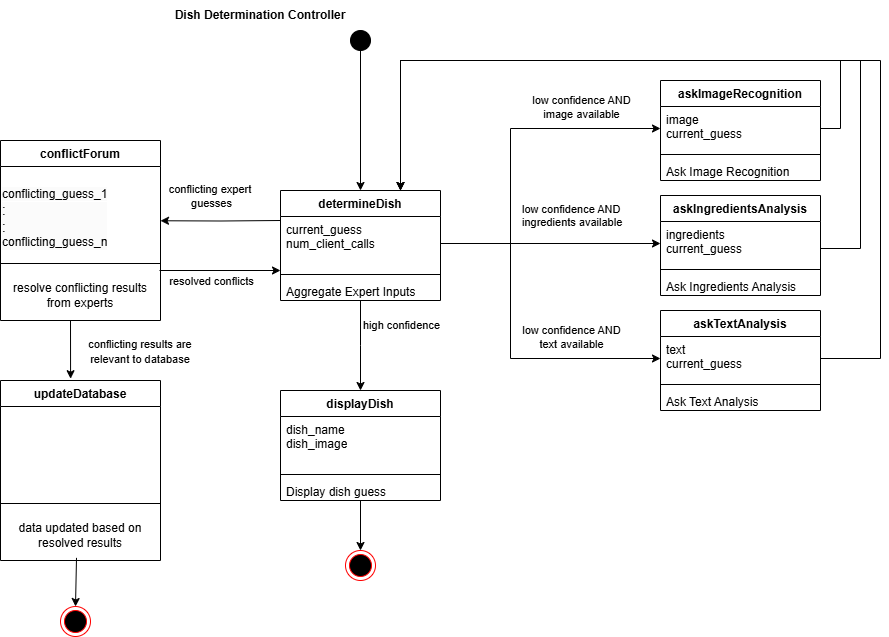
\includegraphics[width=\textwidth]{image/D3_state_diagrams/dish_determination.png}
\end{figure}

\begin{figure}[H]
	\centering
   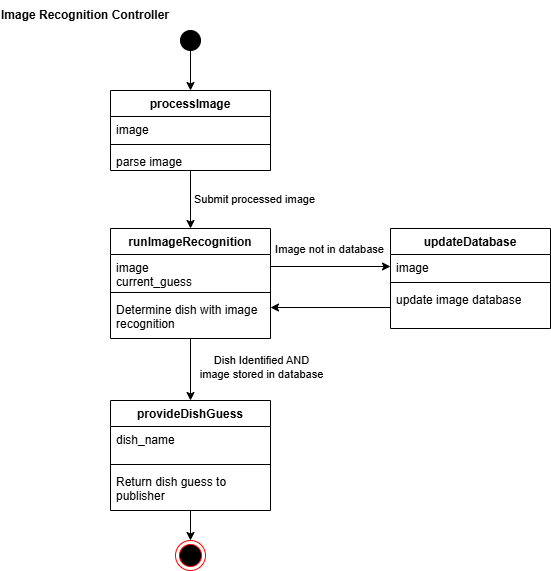
\includegraphics[width=\textwidth]{image/D3_state_diagrams/image_recognition.png}
\end{figure}

\begin{figure}[H]
	\centering
   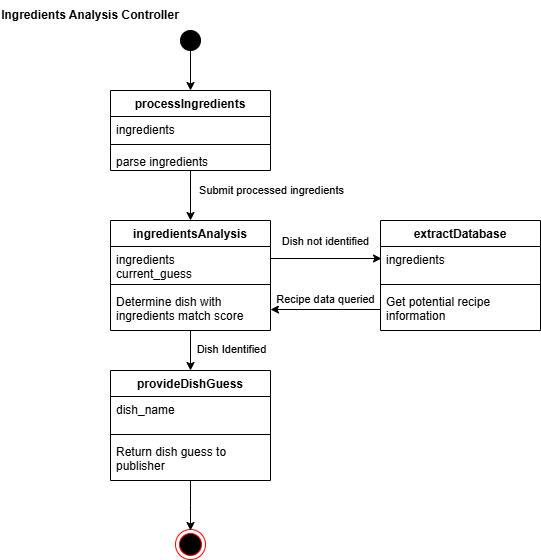
\includegraphics[width=\textwidth]{image/D3_state_diagrams/ingredients_analysis.png}
\end{figure}


\begin{figure}[H]
	\centering
   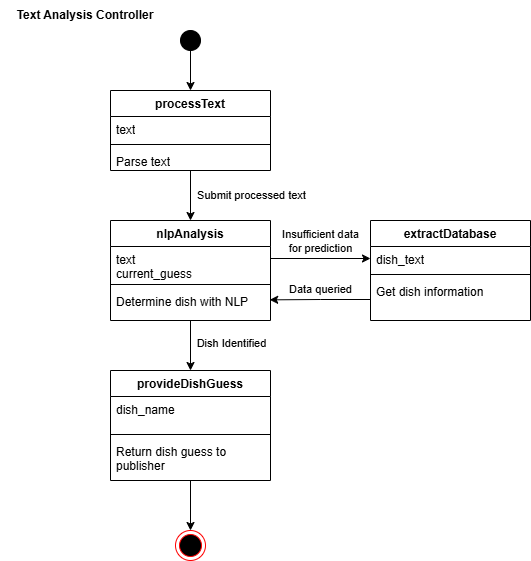
\includegraphics[width=\textwidth]{image/D3_state_diagrams/text_analysis.png}
\end{figure}

\begin{figure}[H]
	\centering
   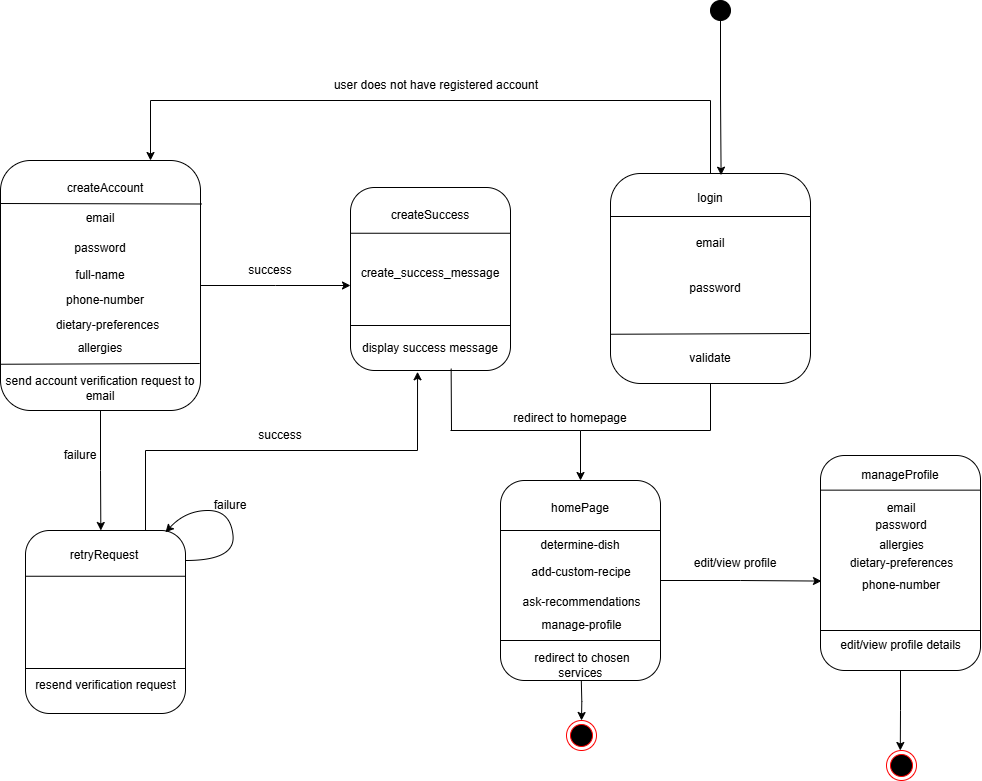
\includegraphics[width=\textwidth]{image/D3_state_diagrams/account_management.png}
\end{figure}

\begin{figure}[H]
	\centering
   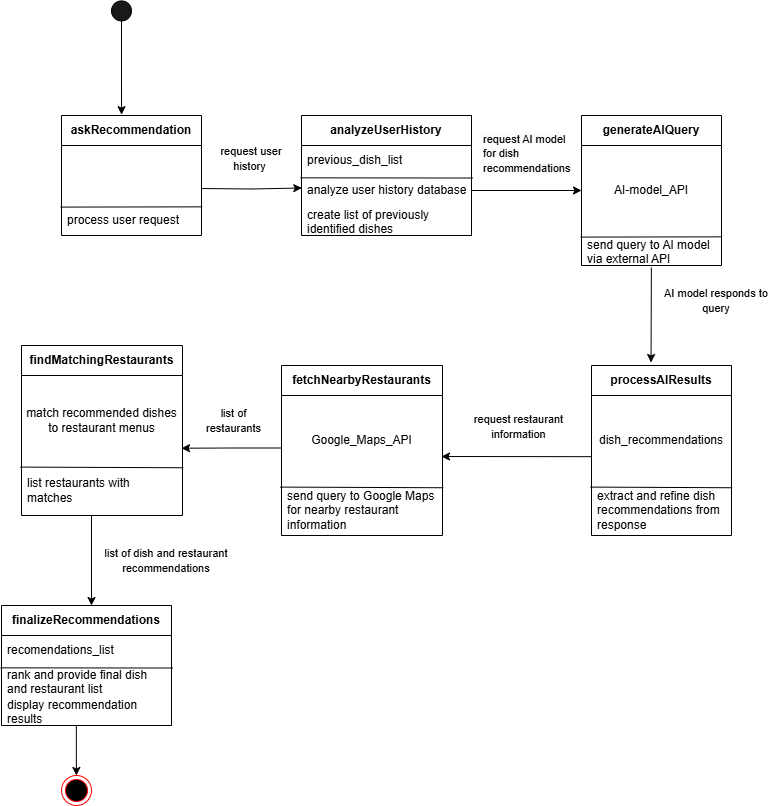
\includegraphics[width=\textwidth]{image/D3_state_diagrams/recommendation_system.png}
\end{figure}

\begin{figure}[H]
	\centering
   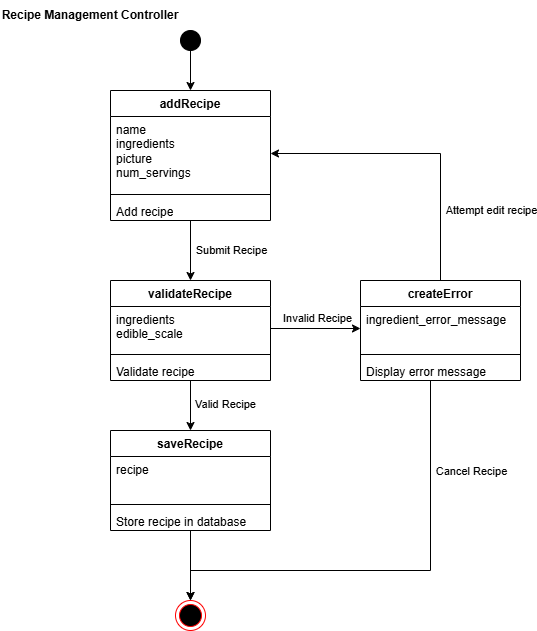
\includegraphics[width=\textwidth]{image/D3_state_diagrams/recipe_management.png}
\end{figure}

% End Section

\section{Sequence Diagrams}
\label{sec:sequence_diagrams}
% Begin Section
This section should provide a sequence diagram for each use case of your application.
% End Section

\section{Detailed Class Diagram}
\label{sec:detailed_class_diagram}
% Begin Section
\begin{figure}[H]
	\centering
   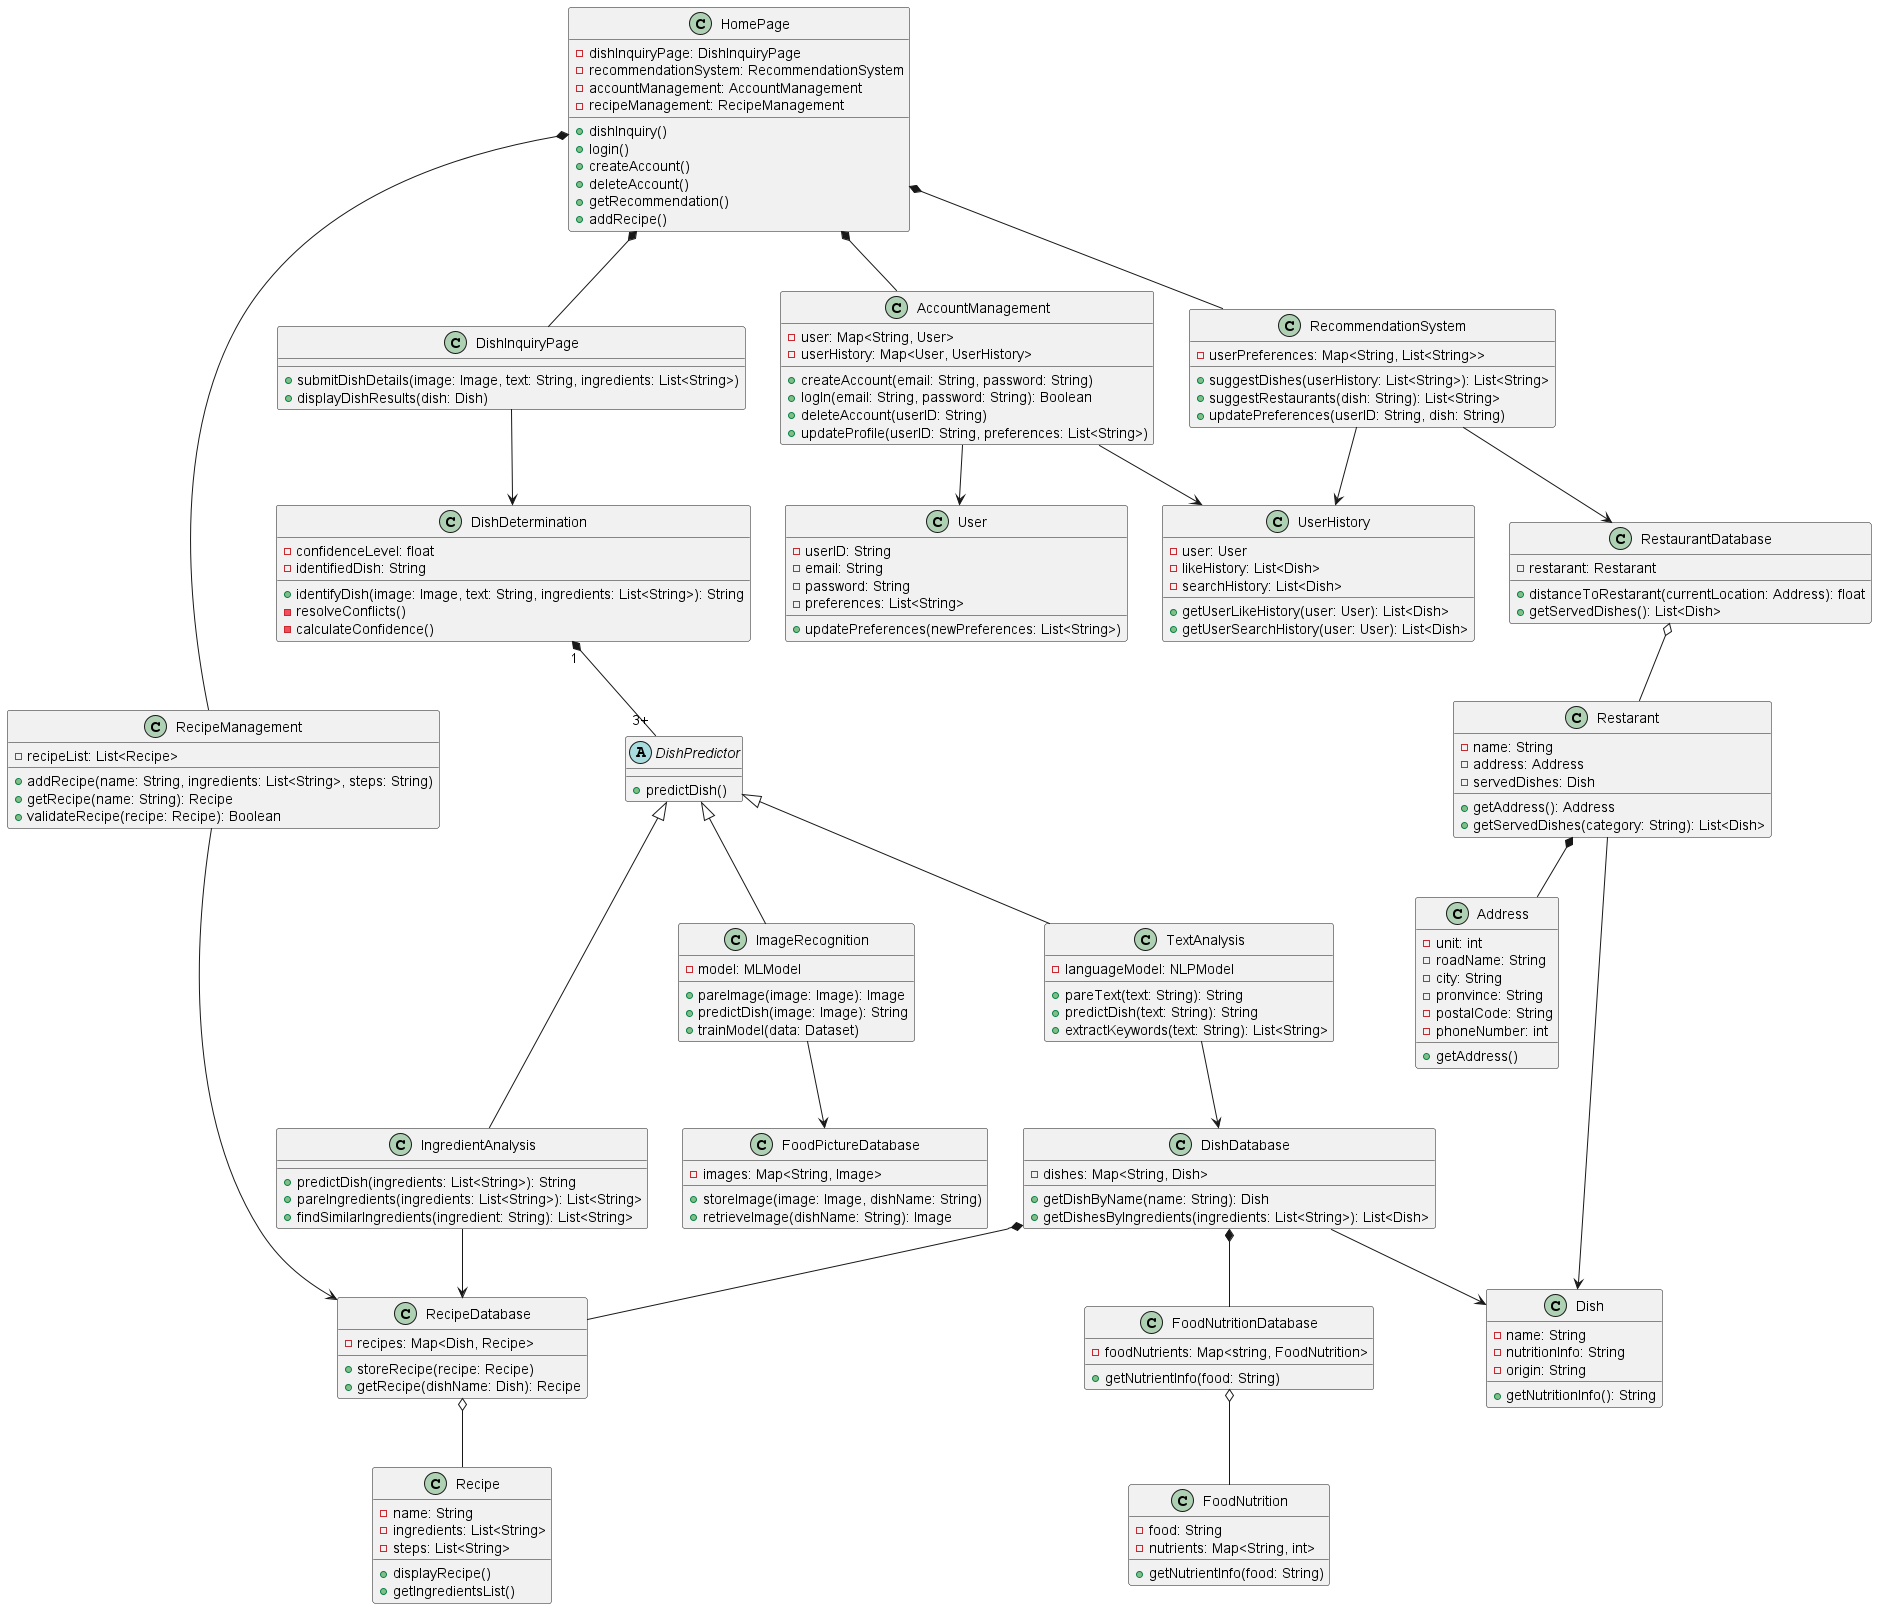
\includegraphics[width=\textwidth]{image/detailedClassDiagram.png}
   \caption{The detailed class diagram}
\end{figure}

\begin{figure}[H]
	\centering
	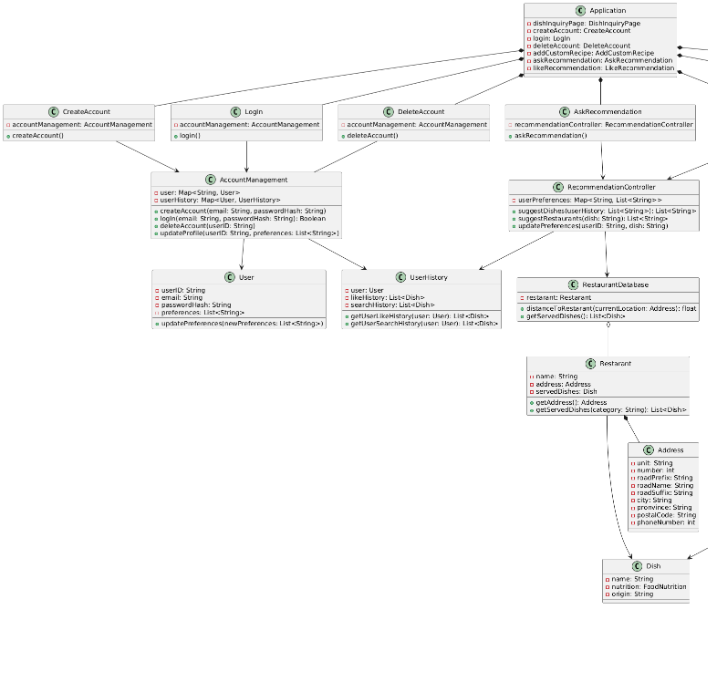
\includegraphics[width=\textwidth]{image/classDiagLeft.png}
	\caption{The view of the detailed class diagram's left side}
\end{figure}

\begin{figure}[H]
	\centering
	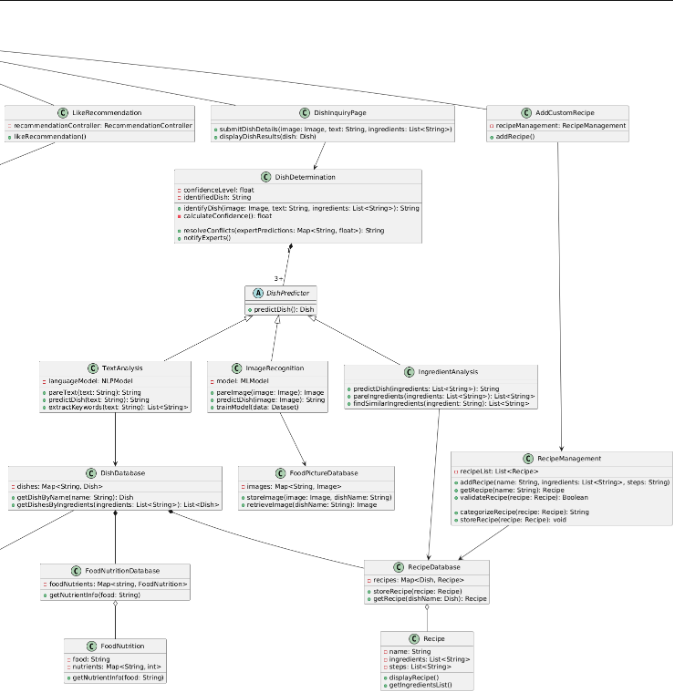
\includegraphics[width=\textwidth]{image/classDiagRight.png}
	\caption{The view of the detailed class diagram's right side}
\end{figure}



% End Section

\appendix
\section{Division of Labour}
\label{sec:division_of_labour}
% Begin Section
\textbf{Imran Chowdhury:}
\begin{enumerate}
	\item TODO
\end{enumerate}

\textbf{Signature:} Imran Chowdhury \\

\textbf{Michael Roberts:}
\begin{enumerate}
	\item Drafted Sections 1.1 and 1.2.
	\item Drafted and revised class diagram with Zifan.
	\item Reviewed section 1.3
	\item Formatted views of the detailed class diagram
\end{enumerate}

\begin{figure}[H]
 	\centering
    
\includegraphics[width=\textwidth]{image/A_Michael_Roberts_Signature.png}
\end{figure}

\textbf{Sathurshan Arulmohan:}
\begin{enumerate}
	\item Developed state diagrams for recipe management, image recognition, text analysis, and ingredients analysis controllers.
	\item Worked with Tanisha on state diagram for dish determination.
	\item Reviewed and provided feedback for state diagrams for recommendation system and account managerment controller.
	\item Edited the detailed class diagram.
	\item Wrote section 1.3.
\end{enumerate}

\textbf{Signature:} SATHURSHAN ARULMOHAN \\

\textbf{Tanisha Tasnin:}
\begin{enumerate}
	\item TODO
\end{enumerate}

\textbf{Signature:} TANISHA TASNIN \\

\textbf{Zifan Si:}
\begin{enumerate}
	\item add part 4 class diagram.
	\item add be1 sequence diagram.
	\item add be6 sequence diagram.
	\item add fix to D2 3.2
	\item add fix to D2 figure error
\end{enumerate}

\textbf{Signature:} ZIFAN SI  \\
% End Section


\end{document}
%------------------------------------------------------------------------------